\begin{appendices}

\chapter{Signed Letter of Informed Consent}

\begin{figure}[H]
    \centering
    \begin{subfigure}{0.3\textwidth}
        \centering
        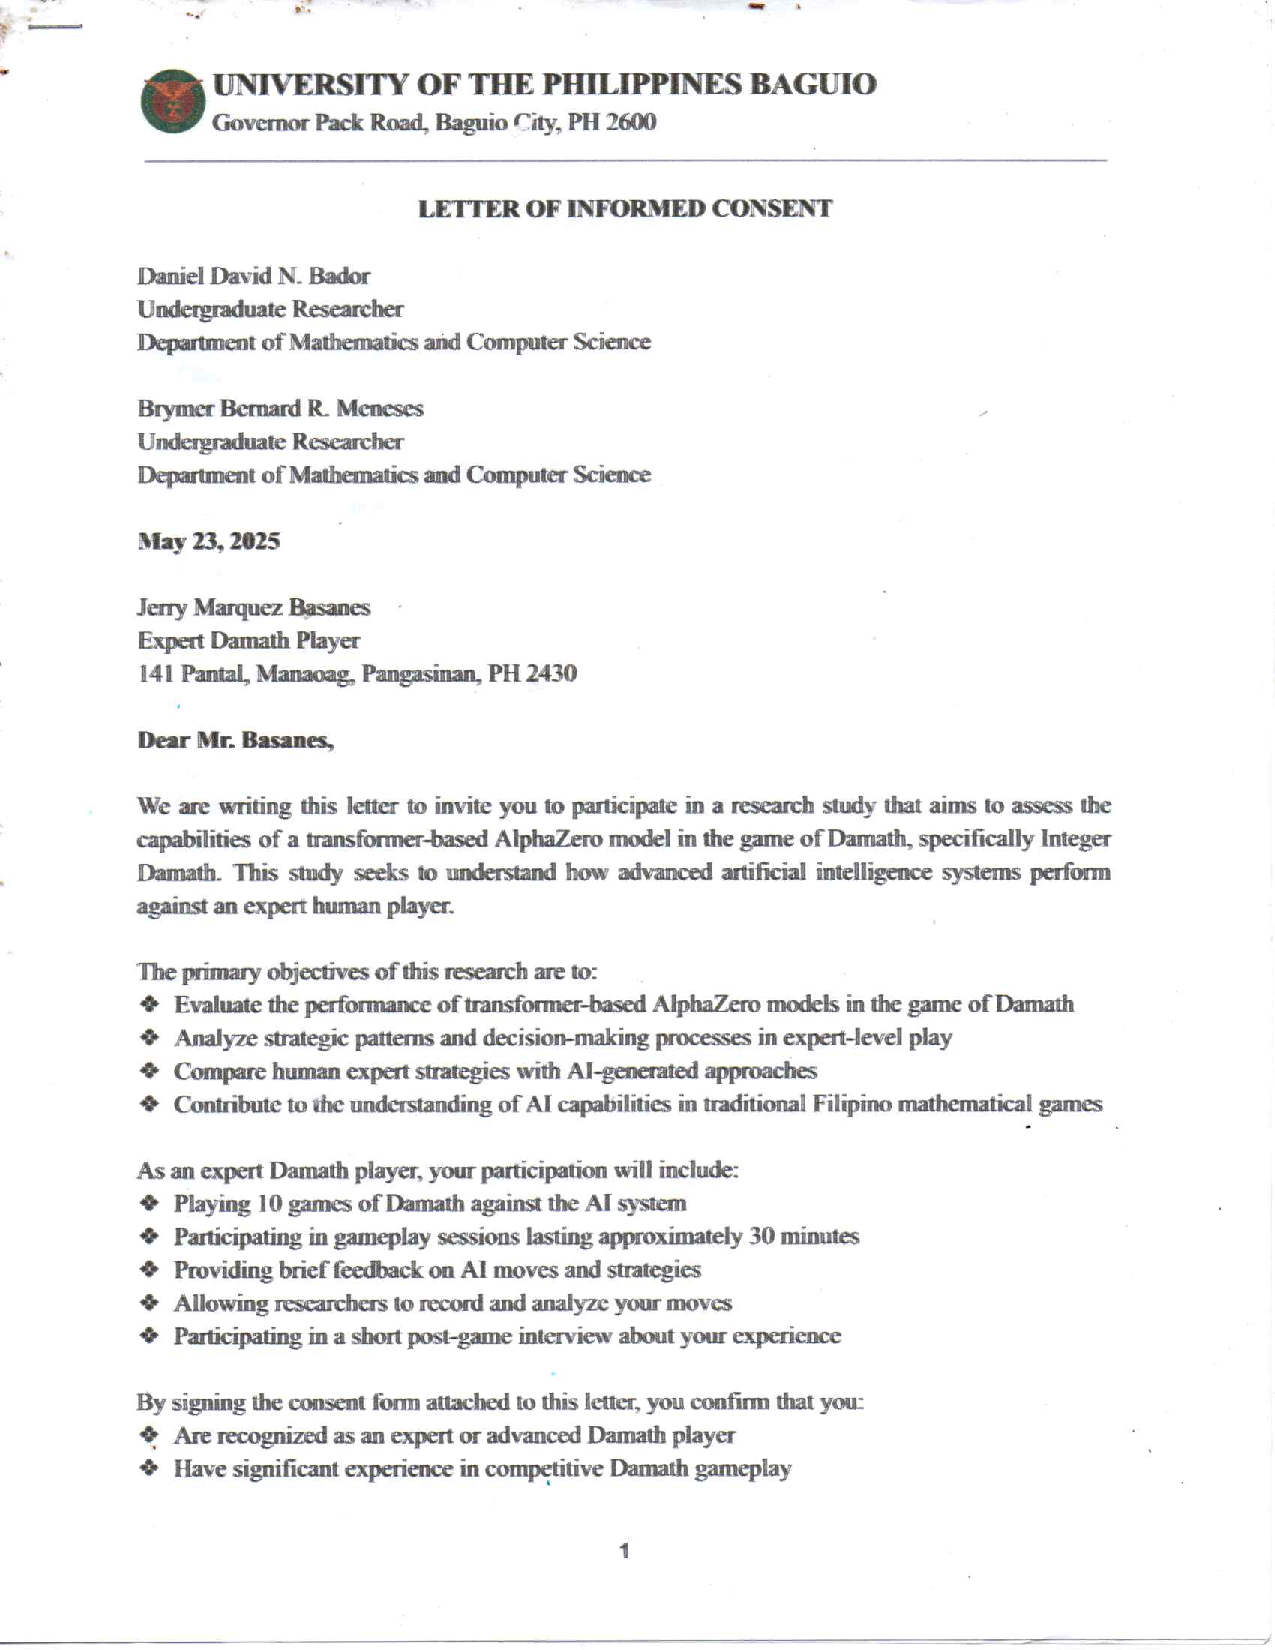
\includegraphics[page=1,width=\linewidth]{images/Letter of Informed Consent.pdf}
    \end{subfigure}
    \begin{subfigure}{0.3\textwidth}
        \centering
        \includegraphics[page=2,width=\linewidth]{images/Letter of Informed Consent.pdf}
    \end{subfigure}
    \begin{subfigure}{0.3\textwidth}
        \centering
        \includegraphics[page=3,width=\linewidth]{images/Letter of Informed Consent.pdf}
    \end{subfigure}
    \caption{Signed Letter of Informed Consent}
    \label{fig:signed-letter-of-informed-consent}
\end{figure}

\chapter{Games Against a Human Player}

\begingroup
\renewcommand\arraystretch{0.75}
\begin{longtable}[H]{cccccc}
    \hline
    \multicolumn{3}{c}{AI}       & \multicolumn{3}{c}{HUMAN}     \\ \hline
    Move         & Score & Total & Move          & Score & Total \\ \hline
      6 to (4,3) &      &  0    &   6 to (3, 4) &      &  0    \\ \hline
      6 to (5,4) &      &  0    &  -9 to (4, 3) & -15   & -15   \\ \hline
     -3 to (3,2) &      &  0    &  -9 to (2, 1) & -12   & -27   \\ \hline
                 &      &  0    &  -9 to (0, 3) &  81   &  54   \\ \hline
      0 to (1,2) &      &  0    &  -9 to (2, 1) &  -9    & 45    \\ \hline
    -11 to (3,2) &  99   &  99   &   6 to (2, 3) &      &  45    \\ \hline
    -11 to (1,4) &  $-5$  &  94  &  -1 to (0, 3) &  11   &  56    \\ \hline
     -1 to (6,3) &      &  94  &  10 to (4, 5) &      &  56    \\ \hline
      8 to (2,1) &      &  94  &  -1 to (1, 2) &      &  56    \\ \hline
      8 to (0,3) &  -8   &  86   &  -7 to (2, 5) &      &  56    \\ \hline
      8 to (1,4) &      &  86   &   4 to (2, 3) &  0.5  &  56.5  \\ \hline
     10 to (5,2) &      &  86   &  -3 to (6, 5) &      &  56.5  \\ \hline
     -1 to (7,4) &      &  86   &  10 to (3, 4) &      &  56.5   \\ \hline
     -1 to (5,6) &  -4   &  82   & -11 to (4, 5) &  11   &  67.5    \\ \hline
     -5 to (4,1) &      &  82   &   4 to (3, 2) &      &  67.5    \\ \hline
     -5 to (2,3) &  -1.25  &  80.75    &  10 to (1, 2) &  -2    &  65.5    \\ \hline
     10 to (4,3) &      &  80.75    &  -7 to (3, 4) &      &  65.5    \\ \hline
     10 to (2,5) &  3    &  83.75    &  10 to (2, 1) &      &  65.5    \\ \hline
     10 to (1,6) &      &  83.75    &   2 to (2, 5) &  12    &  77.5    \\ \hline
     -7 to (5,2) &      &  83.75    &   0 to (6, 5) &      &  77.5    \\ \hline
     -7 to (6,3) &      &  83.75    &  10 to (1, 0) &      &  77.5    \\ \hline
      2 to (6,1) &      &  83.75    &  10 to (5, 4) &      &  77.5    \\ \hline
      2 to (5,2) &      &  83.75    & -11 to (3, 4) &      &  77.5    \\ \hline
     -7 to (4,5) &  -140  &  -56.25  &                &      &  77.5    \\ \hline
     -7 to (2,3) &  $0.\overline{63}$   &  $-55.61\overline{36}$   &   2 to (3,4)  &  0    &  77.5    \\ \hline
     -7 to (4,5) &  -14    &   $-69.61\overline{36}$&  -5 to (3,6)  &      &  77.5    \\ \hline
     -7 to (2,7) &  1.4    &  $-68.21\overline{36}$   &   0 to (5,4)  &      &  77.5    \\ \hline
     -7 to (6,3) &  -14    & $-82.21\overline{36}$     &   8 to (3,6)  &      &  77.5    \\ \hline
     -7 to (2,7) &  -1.75    &  $-83.9\overline{36}$   &               &      &      \\ \hline\hline 
                 &           &  $-91.9\overline{63}$   &               &      & 77.5  \\ \hline 
    \caption{Game Moves of the First Game Against an Expert Damath Player}
    \label{tab:first-game}
\end{longtable}
\endgroup

\begin{table}[H]
    \centering
    \begin{tabular}{cccccc}
        \hline
        \multicolumn{3}{c}{HUMAN}        & \multicolumn{3}{c}{AI}     \\ \hline
        Move         & Score & Total & Move          & Score & Total \\ \hline
          -1 to (3,3) &      &  0    &   -9 to (5, 4) &      &  0    \\ \hline
          -1 to (6,5) & $0.\overline{1}$ &  $0.\overline{1}$  &    0 to (5, 4) & 0      &  0    \\ \hline
          4 to (5,3) &      & $0.\overline{1}$  &    0 to (7, 2) &  $-4$    &  $-4$    \\ \hline
          10 to (5,2) &      &  $0.\overline{1}$    &    -3 to (6, 5) &      &  $-4$    \\ \hline
          -5 to (4,1) &      &  $0.\overline{1}$    &    0 to (5, 0) &  0    &  $-4$    \\ \hline
          6 to (3,3) &      &  $0.\overline{1}$    &    0 to (3, 2) &  0    &  $-4$    \\ \hline
                     &      &  $0.\overline{1}$    &    0 to (5, 4) &  0    &  $-4$    \\ \hline
          10 to (5,3) &      &  $0.\overline{1}$    &    0 to (7, 2) &  $-20$    &  $-24$    \\ \hline
          2 to (6,1) &      &  $0.\overline{1}$    &    0 to (5, 0) &  $0$    &  $-24$    \\ \hline
          -9 to (1,3) &      &  $0.\overline{1}$    &    0 to (1, 4) &  $-18$    &  $-42$    \\ \hline
          0 to (1,2) &      &  $0.\overline{1}$    &    -11 to (5, 6) &      &  $-42$    \\ \hline
          8 to (4,1) &      &  $0.\overline{1}$    &    0 to (5, 0) &  $0$    &  $-42$    \\ \hline
          -3 to (3,2) &      &  $0.\overline{1}$    &    0 to (1, 3) &  $0$    &  $-42$    \\ \hline
                     &      &  $0.\overline{1}$    &    0 to (0, 1) &  $0$    &  $-42$    \\ \hline
          -11 to (2,1) &      &  $0.\overline{1}$    &    0 to (1, 2) &      &  $-42$    \\ \hline
          -11 to (0,3) &  0    &  $0.\overline{1}$    &    -3 to (7, 4) &      &  $-42$    \\ \hline
          -11 to (1,4) &      &  $0.\overline{1}$    &    4 to (2, 3) &  $-0.\overline{36}$    &  $-42.\overline{36}$    \\ \hline \hline
                       &     &   $0.\overline{1}$  &                &          &  $-39.\overline{36}$
    \end{tabular}
    \caption{Game Moves of the Second Game Against an Expert Damath Player}
    \label{tab:second-game}
\end{table}

\begin{table}[H]
    \centering
    \begin{tabular}{cccccc}
        \hline
        \multicolumn{3}{c}{AI}        & \multicolumn{3}{c}{HUMAN}     \\ \hline
        Move         & Score & Total & Move          & Score & Total \\ \hline
          6 to (4,3) &      &  0    &   6 to (3, 4) &      &  0    \\ \hline
          6 to (5,4) &      &  0    &   -9 to (4, 3) &  $-15$    &  $-15$    \\ \hline
          -3 to (3,2) &      &  0    &   -9 to (2, 1) &  $-12$    &  $-27$    \\ \hline
                      &      &  0    &   -9 to (0, 3) &  $81$    &  $54$    \\ \hline
          0 to (1,2) &      &  0    &   -9 to (2, 1) &  $-9$    &  $45$    \\ \hline
          -11 to (3,2) &  99  &  99    &   6 to (2, 3) &      &  $45$    \\ \hline
          -11 to (1,4) &  $-5$   &  94    &   -1 to (0, 3) &  $11$    &  $56$    \\ \hline
          10 to (3,2) &     &  94    &   -7 to (2, 5) &      &  $56$    \\ \hline
          4 to (6,3) &      &  94    &   10 to (4, 5) &      &  $56$    \\ \hline
          10 to (4,3) &      &  94    &   -7 to (3, 4) &      &  $56$    \\ \hline
          10 to (2,5) &  3    &  97    &   -3 to (6, 5) &      &  $56$    \\ \hline
          10 to (1,6) &      &  97    &   2 to (2, 5) &  $12$    &  $68$    \\ \hline
          8 to (4,1) &      &  97    &   -1 to (1, 2) &      &  $68$    \\ \hline
          4 to (7,4) &      &  97    &   -11 to (5, 6) &      &  $68$    \\ \hline
          -7 to (7,2) &      &  97    &   2 to (3, 4) &      &  $68$    \\ \hline
          8 to (3,2) &      &  97    &   2 to (2, 3) &      &  $68$    \\ \hline
          8 to (1,4) &  10    &  107    &   4 to (2, 3) &  $0.5$    &  $68.5$    \\ \hline
          -5 to (4,1) &      &  107    &   -1 to (2, 1) &      &  $68.5$    \\ \hline
          -1 to (4,3) &      &  107    &   10 to (3, 4) &      &  $68.5$    \\ \hline
          -1 to (2,5) &  9    &  116    &   -1 to (1, 0) &      &  $68.5$    \\ \hline
          -5 to (5,2) &      &  116    &   8 to (3, 6) &      &  $68.5$    \\ \hline
          -1 to (4,7) &  $-9$  & 107  0    &   -3 to (5, 4) &      &  $68.5$    \\ \hline
          -1 to (6,5) &  $0.\overline{18}$    & $107.\overline{18}$     &                &      &  $68.5$    \\ \hline
          -1 to (3,2) &  6    &  $113.\overline{18}$    &                &      &  $68.5$    \\ \hline
          -1 to (0,5) &  $-10$    &  $103.\overline{18}$    &   0 to (6,5)   &      &  $68.5$    \\ \hline
          4 to (5,6) &  $4$    &  $107.\overline{18}$    &   -1 to (6,5)   &      &  $68.5$    \\ \hline
          4 to (7,4) &  $-8$    &  $99.\overline{18}$   &   -5 to (1,6)   &      &  $68.5$    \\ \hline
          -1 to (2,7) &  $0.4$    & $99.5\overline{81}$     &                &      &  $68.5$    \\ \hline \hline
           &      & $91.5\overline{81}$     &                &      &  $68.5$    \\ \hline
    \end{tabular}
    \caption{Game Moves of the Third Game Against an Expert Damath Player}
    \label{tab:third-game}
\end{table}


\begin{table}[H]
    \centering
    \begin{tabular}{cccccc}
        \hline
        \multicolumn{3}{c}{AI}        & \multicolumn{3}{c}{HUMAN}     \\ \hline
        Move         & Score & Total & Move          & Score & Total \\ \hline
          -1 to (6,3) &      &  0    &   -1 to (1, 4) &      &  0    \\ \hline
          10 to (5,2) &      &  0    &   -9 to (5, 4) &      &  0    \\ \hline
          6 to (4,3) &      &  0    &   -9 to (3, 2) &  $-54$    &  $-54$    \\ \hline
          -3 to (4,3) &  6    &  6    &   6 to (3, 4) &      &  $-54$    \\ \hline
          -3 to (2,5) &  3    &  9    &               &      &  $-54$    \\ \hline
          -3 to (0,3) &  3    &  12    &   0 to (6,5)        &      &  $-54$    \\ \hline
          -1 to (7,4) &      &  12    &   -7 to (2,5)        &      &  $-54$    \\ \hline
          -3 to (1,4) &      &  12    &   -7 to (0,3)        &  21 &  $-33$    \\ \hline
                      &      &  12    &   -7 to (2,1)        &  $-16$    &  $-49$    \\ \hline
          -11 to (3,2) &  77    &  89    &   10 to (2,5)        &      &  $-49$    \\ \hline
          8 to (2,1) &      &  89    &   8 to (3,6)        &      &  $-49$    \\ \hline
          0 to (1,2) &      &  89    &   2 to (1,6)        &      &  $-49$    \\ \hline
          0 to (0,3) &      &  89    &   0 to (5,4)        &      &  $-49$    \\ \hline
          -11 to (4,3) &      &  89    &   0 to (3,2)        &  $0$    &  $-49$    \\ \hline
                       &      &  89    &   0 to (1,0)        &  8    &  $-41$    \\ \hline
          -1 to (6,5) &      &  89    &   0 to (7,6)        &  2    &  $-39$    \\ \hline
          0 to (1,4) &      &  89    &   10 to (0,3)        &  0    &  $-39$    \\ \hline
          4 to (6,3) &      &  89    &   10 to (1,2)        &      &  $-39$    \\ \hline
          10 to (4,3) &      &  89    &   0 to (2,1)        &  $20$    & $-19$      \\ \hline
          -7 to (5,2) &      &  89    &   0 to (4,3)        &      &  $-19$    \\ \hline
          -7 to (3,4) &  $-14$  & $75$      &   -3 to (4,5)        &     &  $-19$    \\ \hline
          -7 to (5,6) &  $-10$    &  65    &   -11 to (4,5)        &  77    &  58    \\ \hline
          4 to (7,4) &      &  65    &   10 to (0,1)        &      &  58    \\ \hline
          2 to (6,1) &      &  65    &   10 to (1,0)        &      &  58    \\ \hline
          2 to (7,2) &      &  65    &   2 to (2,5)        &      &  58    \\ \hline
          -5 to (4,1) &      &  65    &   2 to (3,4)        &      &  58    \\ \hline
          2 to (6,3) &      &  65    &   -11 to (5,4)        &      &  58    \\ \hline
          2 to (4,5) &  $-22$    &  43    &         &      &  58    \\ \hline
          2 to (2,3) &  1    &  44    &  4 to (1, 4)       &      &  58    \\ \hline
          2 to (0,5) &  $-2$    &  42    &  8 to (2, 5)       &      &  58    \\ \hline
          2 to (1,6) &      &  42    &  8 to (0, 7)       &  16    &  74    \\ \hline
          -5 to (3,2) &      &  42    &  10 to (7, 6)       &  30    &  104    \\ \hline
          4 to (6,5) &      &  42    &  10 to (3, 2)       &  80    &  184    \\ \hline\hline
                     &      &  42    &                     &     &  207    \\ \hline
    \end{tabular}
    \caption{Game Moves of the Fourth Game Against an Expert Damath Player}
    \label{tab:fourth-game}
\end{table}

\begin{table}[H]
    \centering
    \begin{tabular}{cccccc}
        \hline
        \multicolumn{3}{c}{AI}        & \multicolumn{3}{c}{HUMAN}     \\ \hline
        Move         & Score & Total & Move          & Score & Total \\ \hline
          -1 to (6,3) &     &  0    &   6 to (3, 4) &      &  0    \\ \hline
          6 to (2,3) &     &  0    &   10 to (4, 5) &      &  0    \\ \hline
          -1 to (5,4) &     &  0    &   -9 to (4, 3) & $-8$   &  $-8$    \\ \hline
          -3 to (3,2) &     &  0    &   -9 to (2, 1) & $-12$   &  $-20$    \\ \hline
                      &     &  0    &   -9 to (0, 3) & 81   &  $61$    \\ \hline
          0 to (1,2) &      &  0    &   -9 to (2, 1) & $-9$   &  $52$    \\ \hline
          -11 to (3,2) &  99 &  99    & 6 to (1, 2) & $1$   &  $53$    \\ \hline
          10 to (5,2) &   &  99       & 4 to (1, 4) &    &  $53$    \\ \hline
          10 to (6,3) &   &  99       & 4 to (2, 3) &    &  $53$    \\ \hline
          -11 to (1,4) & $-7$   &  92  &            &    &  $53$    \\ \hline
          -11 to (3,6) & $11$   &  103  &            &    &  $53$    \\ \hline
          -11 to (5,4) & $-1.1$   &  $101.9$  & 0 to (6,5)      &    &  $53$    \\ \hline
          -11 to (7,6) & $-11$   &  $90.9$  & 6 to (0,1)      &    &  $53$    \\ \hline
          10 to (7,4) &    &  $90.9$  & $-3$ to (4,5)      &    &  $53$    \\ \hline
          8 to (4,1) &    &  $90.9$  & $6$ to (1,0)      &    &  $53$    \\ \hline
          8 to (3,2) &    &  $90.9$  & $6$ to (5,4)      & 1.5    &  $54.5$    \\ \hline
          4 to (6,3) &    &  $90.9$  & $6$ to (7,2)      & 4    &  $58.5$    \\ \hline
          -5 to (4,1) &    &  $90.9$  & $6$ to (5,0)      & $-1.7143$  &  $56.7857$    \\ \hline
                      &    &  $90.9$  & $6$ to (0,5)      & 22  &  $78.7857$    \\ \hline
          2 to (6,1) &    &  $90.9$  & $8$ to (5,6)      &   &  $78.7857$    \\ \hline
          2 to (7,2) &    &  $90.9$  & $-3$ to (5,4)      &   &  $78.7857$    \\ \hline
          2 to (6,3) &    &  $90.9$  & $-3$ to (7,2)      & $-5$   &  $73.7857$    \\ \hline
          10 to (6,5) &    &  $90.9$  & $8$ to (7,4)      & $80$   &  $153.7857$    \\ \hline\hline
                      &    &  $79.9$  &                   &        &  $149.7857$    \\ \hline
    \end{tabular}
    \caption{Game Moves of the Fifth Game Against an Expert Damath Player}
    \label{tab:fifth-game}
\end{table}

\begin{table}[H]
    \centering
    \begin{tabular}{cccccc}
        \hline
        \multicolumn{3}{c}{AI}        & \multicolumn{3}{c}{HUMAN}     \\ \hline
        Move         & Score & Total & Move          & Score & Total \\ \hline
          -1 to (6,3) &      &  0    &   4 to (1, 4) &      &  0    \\ \hline
          -7 to (5,2) &      &  0    &   -1 to (3, 4) &      &  0    \\ \hline
          6 to (2,3) &       &  0    &   4 to (3, 2) &  24   &  24    \\ \hline
          -3 to (4,3) & $-7$ &  $-7$ &               &       &  24    \\ \hline
          -3 to (2,5) & $-4$ &  $-11$ &  -7 to (3,4) & $-4$ &  20    \\ \hline
          -7 to (4,3) &      &  $-11$ &  -7 to (5,2) & $-14$ &  6    \\ \hline
                      &      &  $-11$ &  -7 to (7,4) & $7$   &  13    \\ \hline
          2 to (6,1)  &      &  $-11$ &  -7 to (6,3) &       &  13    \\ \hline
          4 to (5,4)  & $-0.5714$  &  $-11.5714$ &  6 to (6,3) & 10       &  23    \\ \hline
          -11 to (2,1)  &          &  $-11.5714$ &  6 to (5,2) &          &  23    \\ \hline
          2 to (4,3)  & $-4$       &  $-15.5714$ &  $-9$ to (5,4) &          &  23    \\ \hline
          2 to (6,5)  & $-0.\overline{22}$    &  $-15.57937$ &  $0$ to (5,4) &  0 &  23    \\ \hline
          $-9$ to (2,3)  &    &  $-15.57937$ &  $-3$ to (6,5) &    &  23    \\ \hline
          $10$ to (5,2)  &    &  $-15.57937$ &  $0$ to (4,3) &    &  23    \\ \hline
          $10$ to (3,4)  & 10    &  $-5.57937$ &  $10$ to (4,5) &    &  23    \\ \hline
          $10$ to (5,6)  & 20    &  $14.2063$ &                 &    &  23    \\ \hline
          $10$ to (7,4)  & -30    &  $-15.7937$ & 8 to (5,6)    &    &  23    \\ \hline
          $-5$ to (4,1)  &        &  $-15.7937$ & $-11$ to (7,6) &    &  23    \\ \hline
          $-5$ to (5,2)  &        &  $-15.7937$ & $8$ to (6,5) &    &  23    \\ \hline
          $10$ to (5,6)  & 18     &  $2.2063$   & $-11$ to (6,5) &    &  23    \\ \hline
          $10$ to (7,4)  & -110   &  $-107.7937$ & $-5$ to (3,6) &    &  23    \\ \hline
          $10$ to (6,5)  &        &  $-107.7937$ & $-5$ to (4,5) &    &  23    \\ \hline
          $10$ to (7,6)  &        &  $-107.7937$ & $2$ to (1,6) &    &  23    \\ \hline
          $8$ to (4,1)  &        &  $-107.7937$ & $2$ to (0,5) &    &  23    \\ \hline
          $-9$ to (3,4)  &        &  $-107.7937$ & $-5$ to (2,3) & $0.\overline{5}$    &  $23.\overline5$   \\ \hline
          $0$ to (1,2)  &        &  $-107.7937$ & $-5$ to (0,1) & $-5$    &  $18.\overline5$   \\ \hline
          $10$ to (6,7) &        &  $-107.7937$ & $-5$ to (1,0) &         &  $18.\overline5$   \\ \hline
          $-5$ to (4,3) &        &  $-107.7937$ & $-5$ to (3,2) & $110$     &  $128.\overline5$   \\ \hline
                        &        &  $-107.7937$ & $-5$ to (7,6) & $0$       &  $128.\overline5$   \\ \hline
          $10$ to (4,5) &        &  $-107.7937$ & $-5$ to (3,2) &           &  $128.\overline5$   \\ \hline
          $8$ to (2,3) & $-3.2$  &  $-110.9937$ & $2$ to (1,4) &           &  $128.\overline5$   \\ \hline
          $8$ to (0,5) & 6       &  $-104.9937$ &              &           &  $128.\overline5$   \\ \hline \hline
                       &         &  $-76.9937$ &             &           &  $128.\overline5$   \\ \hline
    \end{tabular}
    \caption{Game Moves of the Sixth Game Against an Expert Damath Player}
    \label{tab:sixth-game}
\end{table}

\begin{table}[H]
    \centering
    \begin{tabular}{cccccc}
        \hline
        \multicolumn{3}{c}{HUMAN}        & \multicolumn{3}{c}{AI}     \\ \hline
        Move         & Score & Total & Move          & Score & Total \\ \hline
         $-1$ to (3,3) &       &  0    &   6 to (3, 4) &       &  0    \\ \hline
         $-7$ to (5,2) &       &  0    &   $-3$ to (4, 5) &       &  0    \\ \hline
         $-7$ to (5,3) &       &  0    &   $6$ to (5, 2) & $5$    &  5    \\ \hline
                       &       &  0    &   $6$ to (7, 4) & $-42$    &  $-37$  \\ \hline
         $6$ to (3,3)  &       &  0    &   $8$ to (5, 6) &        &  $-37$    \\ \hline
         $6$ to (5,4)  &       &  0    &   $-3$ to (5, 3) & $3$    &  $-34$    \\ \hline
         $4$ to (5,4)  & $-1.\overline3$ &  $-1.\overline3$   &   $-9$ to (3, 3) & $-13$    &  $-47$    \\ \hline
         $-3$ to (3,2)  &       &  $-1.\overline3$    &   $-9$ to (2, 1) & $-12$    &  $-59$    \\ \hline
                        &       &  $-1.\overline3$    &   $-9$ to (0, 3) & $81$    &  $22$    \\ \hline
         $0$ to (1,2)  &       &  $-1.\overline3$     &   $-9$ to (2, 1) & $-9$    &  $13$    \\ \hline
         $-11$ to (3,2)  &   99 &  $97.\overline6$     &   $0$ to (6, 5) &         &  $13$    \\ \hline
         $10$ to (5,2)  &       &  $97.\overline6$     &   $-1$ to (3, 4) &         &  $13$    \\ \hline
         $-11$ to (1,3)  &       &  $97.\overline6$     &   $-1$ to (1, 2) & $0.\overline{09}$ &  $13.\overline{09}$    \\ \hline
         $8$ to (2,1)  &       &  $97.\overline6$     &   $-1$ to (3, 0) & $-9$ &  $4.\overline{09}$    \\ \hline
         $2$ to (6,1)  &       &  $97.\overline6$     &   $-1$ to (5, 3) & $18$ &  $22.\overline{09}$    \\ \hline
         $-5$ to (4,1)  &       &  $97.\overline6$     &   $-1$ to (3, 0) & 8 &  $30.\overline{09}$    \\ \hline
         $2$ to (5,2)  &        &  $97.\overline6$     &   $-1$ to (5, 3) & 2 &  $32.\overline{09}$    \\ \hline \hline
                       &        &  $97.\overline6$     &                  &   &  $37.\overline{09}$    \\ \hline
    \end{tabular}
    \caption{Game Moves of the Seventh Game Against an Expert Damath Player}
    \label{tab:seventh-game}
\end{table}

\begin{table}[H]
    \centering
    \begin{tabular}{cccccc}
        \hline
        \multicolumn{3}{c}{HUMAN}        & \multicolumn{3}{c}{AI}     \\ \hline
        Move         & Score & Total & Move          & Score & Total \\ \hline
          6 to (3,3) &       &  0    &   6 to (5, 4) &       &  0    \\ \hline
          10 to (3,2) &       &  0    &   6 to (5, 3) &       &  0    \\ \hline
          4 to (5,4) & $0.\overline6$ &  $0.\overline6$    &   $-5$ to (7, 4) &       &  0    \\ \hline
          $-1$ to (5,3) &             &  $0.\overline6$    &   $-9$ to (5, 2) & $-10$       &  $-10$    \\ \hline
                        &             &  $0.\overline6$    &   $-9$ to (3, 4) & $-15$       &  $-25$    \\ \hline
          $-9$ to (1,3) &             &  $0.\overline6$    &   $-9$ to (1, 2) & $1$       &  $-24$    \\ \hline
          $-3$ to (0,3) & $27$        &  $27.\overline6$    &   $0$ to (6, 5) &           &  $-24$    \\ \hline
          $4$ to (7,6)  & $4$        &  $31.\overline6$     &   $10$ to (4, 5) &           &  $-24$    \\ \hline
          $-7$ to (5,2)  &          &  $31.\overline6$     &   $8$ to (3, 6) &           &  $-24$    \\ \hline
          $0$ to (1,2)  &           &  $31.\overline6$     &   $-1$ to (3, 4) &           &  $-24$    \\ \hline
          $-7$ to (3,3)  &           &  $31.\overline6$     &   $-1$ to (5, 2) & $-8$           &  $-32$    \\ \hline
          $2$ to (6,1)  &           &  $31.\overline6$     &   $-1$ to (7, 0) & $-2$           &  $-34$    \\ \hline
          $10$ to (3,3)  &          &  $31.\overline6$     &   $-1$ to (3, 4) & $-22$           &  $-56$    \\ \hline
                         &          &  $31.\overline6$     &   $-1$ to (0, 1) & $-2$           &  $-58$    \\ \hline
          $-3$ to (1,4)  &          &  $31.\overline6$     &   $4$ to (1, 3) & $-1.\overline3$    &  $-59.\overline3$    \\ \hline
          $8$ to (2,1)  &          &  $31.\overline6$     &   $10$ to (3, 4) &                    &  $-59.\overline3$    \\ \hline
          $-5$ to (4,1)  &          &  $31.\overline6$     &   $-3$ to (6, 5) &                    &  $-59.\overline3$    \\ \hline
          $4$ to (5,4)  & $-1.\overline3$  &  $30.\overline3$    &   $-11$ to (5, 6) &                    &  $-59.\overline3$    \\ \hline
          $4$ to (6,5)  &                  &  $30.\overline3$    &   $-11$ to (7, 4) & $-44$                    &  $-103.\overline3$    \\ \hline
          $-5$ to (3,2)  &                  &  $30.\overline3$    &   $4$ to (4, 1) & $-20$                    &  $-123.\overline3$    \\ \hline
          $8$ to (1,2)  &                  &  $30.\overline3$    &   $-1$ to (1, 3) & $-0.25$                    &  $-123.58\overline3$    \\ \hline
          $-11$ to (0,1)  &                  &  $30.\overline3$    &   $-1$ to (0, 5) &                            &  $-123.58\overline3$    \\ \hline
          $-11$ to (1,2)  &                  &  $30.\overline3$    &   $-1$ to (1, 3) &                            &  $-123.58\overline3$    \\ \hline
          $-11$ to (0,3)  &                  &  $30.\overline3$    &   $-7$ to (1, 4) &                            &  $-123.58\overline3$    \\ \hline
          $-11$ to (1,4)  &                  &  $30.\overline3$    &   $4$ to (3, 0) &                            &  $-123.58\overline3$    \\ \hline
          $-11$ to (3,2)  & $22$                  &  $52.\overline3$    &   $4$ to (2, 1) &                            &  $-123.58\overline3$    \\ \hline
          $-11$ to (1,0)  & $-14$                  &  $38.\overline3$    &   $-11$ to (5, 3) &                            &  $-123.58\overline3$    \\ \hline
          $-11$ to (2,1)  &                        &  $38.\overline3$    &   $-11$ to (7, 2) &                            &  $-123.58\overline3$    \\ \hline
          $-11$ to (3,2)  &                        &  $38.\overline3$    &   $10$ to (3, 3) &                            &  $-123.58\overline3$    \\ \hline
          $-11$ to (5,4)  & $-1.1$                        &  $37.2\overline3$    &   $8$ to (4, 5) &                            &  $-123.58\overline3$    \\ \hline
          $-11$ to (3,6)  & $-88$                        &  $-50.7\overline6$    &   $-5$ to (4, 5) &            $55$ &  $-68.58\overline3$    \\ \hline \hline
                          &                              &  $-50.7\overline6$    &                  &           &  $-89.58\overline3$    \\ \hline \hline
    \end{tabular}
    \caption{Game Moves of the Eighth Game Against an Expert Damath Player}
    \label{tab:eighth-game}
\end{table}

\begin{table}[H]
    \centering
    \begin{tabular}{cccccc}
        \hline
        \multicolumn{3}{c}{HUMAN}        & \multicolumn{3}{c}{AI}     \\ \hline
        Move         & Score & Total & Move          & Score & Total \\ \hline
          $-9$ to (0,3) &                 &  0    &   $-1$ to (1, 4) &       &  0    \\ \hline
          $-9$ to (2,5) & $-10$           &  $-10$ &   $10$ to (1, 4) & $1$  &  $1$    \\ \hline
          $6$ to (3,3)  &                 &  $-10$ &   $-9$ to (5, 4) &      &  $1$    \\ \hline
          $6$ to (6,5)  & $-0.\overline6$ &  $-10.\overline6$ &   $0$ to (5, 4) & $0$      &  $1$    \\ \hline
          $4$ to (5,3)  &                 &  $-10.\overline6$ &   $0$ to (7, 2) & $-4$      &  $-3$    \\ \hline
          $10$ to (3,2)  &                &  $-10.\overline6$ &   $-11$ to (7, 6) &           &  $-3$    \\ \hline
          $0$ to (1,2)  &                &  $-10.\overline6$ &   $10$ to (0, 3) &           &  $-3$    \\ \hline
          $-5$ to (4,1)  &                &  $-10.\overline6$ &   $0$ to (5, 0) & $0$        &  $-3$    \\ \hline
          $10$ to (3,3)  &                &  $-10.\overline6$ &   $0$ to (3, 2) & $0$        &  $-3$    \\ \hline
                         &                &  $-10.\overline6$ &   $0$ to (5, 4) & $0$        &  $-3$    \\ \hline
          $-1$ to (5,3)  &                &  $-10.\overline6$ &   $0$ to (7, 2) & $2$        &  $-1$    \\ \hline
          $2$ to (6,1)  &                &  $-10.\overline6$ &   $0$ to (5, 0) & $0$        &  $-1$    \\ \hline
          $0$ to (1,3)  &                &  $-10.\overline6$ &   $0$ to (1, 4) & $0$        &  $-1$    \\ \hline
          $-3$ to (1,2)  &                &  $-10.\overline6$ &   $10$ to (2, 1) & $7$        &  $6$    \\ \hline
          $8$ to (1,2)  & $0.8$           &  $-9.8\overline6$ &   $0$ to (5, 0) &            &  $6$    \\ \hline
          $8$ to (0,3)  &                 &  $-9.8\overline6$ &   $0$ to (4, 1) &            &  $6$    \\ \hline
          $-11$ to (0,1)  &               &  $-9.8\overline6$ &   $0$ to (5, 3) &            &  $6$    \\ \hline
          $8$ to (1,4)  &                  &  $-9.8\overline6$ &   $4$ to (1, 3) & $0.5$      &  $6.5$    \\ \hline
          $-11$ to (1,2)  &                &  $-9.8\overline6$ &   $4$ to (0, 1) & $15$      &  $21.5$    \\ \hline \hline
                          &                &  $-9.8\overline6$ &                 &           &  $15.5$    \\ \hline \hline
    \end{tabular}
    \caption{Game Moves of the Ninth Game Against an Expert Damath Player}
    \label{tab:ninth-game}
\end{table}

\begin{table}[H]
    \centering
    \begin{tabular}{cccccc}
        \hline
        \multicolumn{3}{c}{HUMAN}        & \multicolumn{3}{c}{AI}     \\ \hline
        Move         & Score & Total & Move          & Score & Total \\ \hline
          4 to (5,3) &       &  0    &   6 to (3, 4) &       &  0    \\ \hline
          4 to (5,4) &       &  0    &   $-5$ to (3, 3) & $-13$       &  $-13$    \\ \hline
          6 to (5,4) & $-0.\overline6$  &  $-0.\overline6$  & $6$ to (1, 3) &        &  $-13$    \\ \hline
          $-9$ to (3,4) & $-15$  &  $-15.\overline6$  & $-1$ to (3, 3) & $8$        &  $-5$    \\ \hline
                        &        &  $-15.\overline6$  & $-1$ to (6, 5) & $-0.1\overline6$        &  $-5.1\overline6$    \\ \hline
          $10$ to (3,2) &        &  $-15.\overline6$  & $10$ to (4, 5) &            &  $-5.1\overline6$    \\ \hline
          $-7$ to (7,2) &        &  $-15.\overline6$  & $8$ to (3, 6) &            &  $-5.1\overline6$    \\ \hline
          $0$ to (1,2) &          &  $-15.\overline6$  & $8$ to (2, 5) &            &  $-5.1\overline6$    \\ \hline
          $0$ to (0,3) &          &  $-15.\overline6$  & $-1$ to (5, 4) &           &  $-5.1\overline6$    \\ \hline
          $-7$ to (5,3) &          &  $-15.\overline6$  & $-1$ to (7, 2) & $6$           &  $0.8\overline3$    \\ \hline
          $2$ to (6,1) &          &  $-15.\overline6$  & $4$ to (1, 4) &               &  $0.8\overline3$    \\ \hline
          $-3$ to (1,2) &          &  $-15.\overline6$  & $0$ to (6, 5) &               &  $0.8\overline3$    \\ \hline
          $-5$ to (4,1) &          &  $-15.\overline6$  & $-1$ to (5, 0) & $-0.5$       &  $0.\overline3$    \\ \hline
          $-11$ to (2,1) &         &  $-15.\overline6$  & $-1$ to (6, 1) &              &  $0.\overline3$    \\ \hline
          $-1$ to (7,0) & 2        &  $-13.\overline6$  & $-7$ to (0, 5) &              &  $0.\overline3$    \\ \hline
          $-5$ to (5,2) &          &  $-13.\overline6$  & $-11$ to (7, 6) &              &  $0.\overline3$    \\ \hline
          $10$ to (1,3) &          &  $-13.\overline6$  & $4$ to (3, 2) & $40$            &  $40.\overline3$    \\ \hline
                        &          &  $-13.\overline6$  & $4$ to (1, 0) & $-7$             &  $33.\overline3$    \\ \hline
          $8$ to (2,1) &          &  $-13.\overline6$  & $4$ to (3, 3) & $-8$          &  $25.\overline3$    \\ \hline
                       &          &  $-13.\overline6$  & $4$ to (6, 1) & $-1.6$          &  $23.7\overline3$    \\ \hline
          $-1$ to (5,2) & $6$     &  $-7.\overline6$  & $-5$ to (3, 6) &               &  $23.7\overline3$    \\ \hline
          $-3$ to (1,3) &         &  $-7.\overline6$  & $10$ to (5, 4) &               &  $23.7\overline3$    \\ \hline
          $-1$ to (3,3) &         &  $-7.\overline6$  & $10$ to (3, 2) & $-10$           &  $13.7\overline3$    \\ \hline
                        &         &  $-7.\overline6$  & $10$ to (1, 4) & $7$              &  $20.7\overline3$    \\ \hline \hline
                        &         &  $-7.\overline6$  &                &                  &  $14.7\overline3$    \\ \hline
    \end{tabular}
    \caption{Game Moves of the Tenth Game Against an Expert Damath Player}
    \label{tab:tenth-game}
\end{table}
\end{appendices}
